\documentclass{article}
\usepackage{tikz}
\usepackage{braids}

\begin{document}
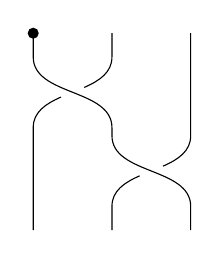
\begin{tikzpicture}
\braid (mybraid) at (3,0) s_1 s_2;
\fill (3,0) circle[radius=2pt];
\end{tikzpicture}

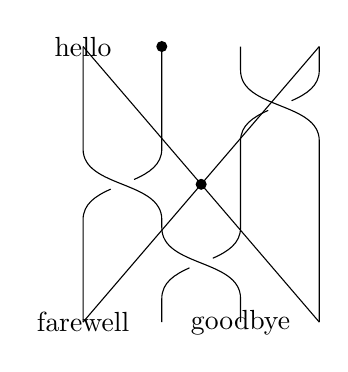
\begin{tikzpicture}
\braid (mybraid) a_3 s_1 s_2;
\node at (mybraid-1-s) {hello};
\node at (mybraid-1-e) {goodbye};
\fill (mybraid-rev-1-s) circle[radius=2pt];
\node at (mybraid-rev-1-e) {farewell};
\fill (mybraid) circle[radius=2pt];
\draw (mybraid-1-s) -- (mybraid-rev-4-e);
\draw (mybraid-4-s) -- (mybraid-rev-1-e);
\end{tikzpicture}


\begin{tikzpicture}
\braid[line width=2pt,style strand={1}{red},style strand={2}{blue},style strand={3}{green}] s_1 s_2^{-1} s_1 s_2^{-1} s_1 s_2^{-1};
\end{tikzpicture}

\begin{tikzpicture}
\braid[
  style floors={fill=yellow},
  style floor={1}{dashed,fill=yellow!50!green},
  floor command={%
    \fill (\floorsx,\floorsy) rectangle (\floorex,\floorey);
    \draw (\floorsx,\floorsy) -- (\floorex,\floorsy);
  },
  line width=2pt,
  style strand={1}{red},
  style strand={2}{blue},
  style strand={3}{green}
]| s_1-s_3-s_5 | s_2^{-1}-s_4| s_1-s_4 s_2^{-1} s_1-s_3 s_2^{-1}-s_4^{-1};
\end{tikzpicture}
\end{document}